% This must be in the first 5 lines to tell arXiv to use pdfLaTeX, which is strongly recommended.
\pdfoutput=1
% In particular, the hyperref package requires pdfLaTeX in order to break URLs across lines.

\documentclass[11pt]{article}

% Change "review" to "final" to generate the final (sometimes called camera-ready) version.
% Change to "preprint" to generate a non-anonymous version with page numbers.
\usepackage[review]{acl}

% Standard package includes
\usepackage{times}
\usepackage{latexsym}
\usepackage{subfigure}
\usepackage{graphicx}
\usepackage{color}
\usepackage{amsmath}
\usepackage{amsfonts}
\usepackage{makecell}
\usepackage{algorithm}
\usepackage{algpseudocode}
\usepackage{multicol}
\usepackage{multirow}

\usepackage{booktabs}
\usepackage{enumitem}
% For proper rendering and hyphenation of words containing Latin characters (including in bib files)
\usepackage[T1]{fontenc}
% For Vietnamese characters
% \usepackage[T5]{fontenc}
% See https://www.latex-project.org/help/documentation/encguide.pdf for other character sets

% This assumes your files are encoded as UTF8
\usepackage[utf8]{inputenc}

% This is not strictly necessary, and may be commented out,
% but it will improve the layout of the manuscript,
% and will typically save some space.
\usepackage{microtype}

% This is also not strictly necessary, and may be commented out.
% However, it will improve the aesthetics of text in
% the typewriter font.
\usepackage{inconsolata}
\newcommand{\secref}[1]{Section~\ref{#1}}
\newcommand{\figref}[1]{Figure~\ref{#1}}
\newcommand{\eqnref}[1]{Eq.~(\ref{#1})}
\newcommand{\tabref}[1]{Table~\ref{#1}}
\newcommand{\exref}[1]{Example~\ref{#1}}
\newcommand{\KZ}[1]{\textcolor{blue}{[Kenny: #1]}}
\newcommand{\Kaiqi}[1]{\textcolor{red}{[Kaiqi: #1]}}
\newcommand{\lawgraph}[1]{Law Graph#1}

% If the title and author information does not fit in the area allocated, uncomment the following
%
%\setlength\titlebox{<dim>}
%
% and set <dim> to something 5cm or larger.

\title{Towards Accurate Prison Term Prediction: A Statute Knowledge Enhanced Approach}

% Author information can be set in various styles:
% For several authors from the same institution:
% \author{Author 1 \and ... \and Author n \\
%         Address line \\ ... \\ Address line}
% if the names do not fit well on one line use
%         Author 1 \\ {\bf Author 2} \\ ... \\ {\bf Author n} \\
% For authors from different institutions:
% \author{Author 1 \\ Address line \\  ... \\ Address line
%         \And  ... \And
%         Author n \\ Address line \\ ... \\ Address line}
% To start a separate ``row'' of authors use \AND, as in
% \author{Author 1 \\ Address line \\  ... \\ Address line
%         \AND
%         Author 2 \\ Address line \\ ... \\ Address line \And
%         Author 3 \\ Address line \\ ... \\ Address line}

\author{First Author \\
  Affiliation / Address line 1 \\
  Affiliation / Address line 2 \\
  Affiliation / Address line 3 \\
  \texttt{email@domain} \\\And
  Second Author \\
  Affiliation / Address line 1 \\
  Affiliation / Address line 2 \\
  Affiliation / Address line 3 \\
  \texttt{email@domain} \\}

\begin{document}
\maketitle
\begin{abstract}
%\begin{abstract}
%  In the age of information explosion, search engines have been an
%  essential tool in people's daily life and query suggestion is one
%  of most useful feature for a standard search engine. However, because
%  most of search engines are keyword-based, many fantastic features would
%  fail when facing concept-based queries, so does query suggestion. In this
%  paper, we propose a framework so that search engines can give acceptable
%  suggestions when facing concept-based queries.
%\end{abstract}

\begin{abstract}
  A class of search queries which contain abstract concepts are studied in
this paper. These queries cannot be correctly interpreted by traditional keyword-based search engines.
  This paper presents a simple framework that detects and instantiates the
abstract concepts by their concrete entities or meanings to produce alternate
queries that yield better search results.
\footnote{Kenny Q. Zhu (corresponding author) is partially
supported by NSFC grants 61100050 and 61033002.}
\end{abstract}

\end{abstract}

\section{Introduction}

Protein$-$protein interactions (PPIs) are of central importance for the majority of biological functions, such as signal transduction, metabolic pathways, molecular dynamics, and protein networks\cite{Hoffmann.Krallinger.ea:2005}, for they serve as the most fundamental building blocks of the entire interacademic systems of any organisms. Collecting data on pairwise interaction relationships is essential for multiple purpose, including identification of modules with certain functionality\cite{Spirin.Mirny.03}, mapping diseases to dominated genes\cite{Ideker.Sharan.08}, and after all, understanding wholistic metabolic/genetic networks from a system biology perspective.

A lot of databases have been built to store protein and genetic interactions from major model organism species and are available in various standardized formats, such as MINT\cite{Zanzoni.Montecchi-Palazzi.ea:2002}, BIND\cite{Bader.ea:2003}, BIOGRID\cite{DBLP:journals/nar/StarkBRBBT06}, etc. Among those mainstream databases, the data largely rely on voluntary reports by scientists or researchers, besides, comprehensive curation efforts become indispensable for the sake of accuracy. However, the amount of biology-related literatures with respect to protein interactions grows explosively and thus make it either impossible or impractical to manually detect PPI information anymore.

Considering huge amount of PPI information with great wealth hidden in published papers, in recent years, numerous mining techniques have been proposed that aim to extract PPI information automatically from free text, especially machine learning, information retrieval, and natural language processing\cite{DBLP:journals/bib/WinnenburgWPDS08}.These approaches can be roughly categorized into three classes: co$-$occurrence, rule$-$based, and machine learning. 

Co$-$occurrence is the approach with most simplicity and naivete. Just as its name implies, this method intends to find out pairs of proteins that co-occur in the same context. The scope of "same context" ranges from phrase, sentence, paragraph to whole abstract, even document. The underlying assumption is that whenever two proteins are mentioned together by authors, chances are high that there is some kind of relationship between them. However, however, in-context closeness even semantic relation does not necessarily represent actual biological interaction. As a consequence, a large fraction of candidate pairs are mismatched inevitably, causing a high recall but low precision.

The second approach is rule-based extraction, in other words, pattern matching. There are many types of rules, most of them concern natural language processing (NLP). One way is to specify hand-crafted regular expressions before hand, which mostly lean on language usage preference. Besides, by using full or partial (shallow) parsing strategies, more information would be acquired, such as part-of-speech taggers, local dependencies between syntactic components, context-free grammar\cite{DBLP:journals/bioinformatics/TemkinG03}, and full sentence structure. Compared to co$-$occurrence, rule-based approach enjoy better precision but much lower recall. In addition, since the rules are usually derived from training data, that is to say, the improper choice of training data would be significantly lethal, therefore quality of extraction is invariably instable and may not applicable to other data.

The third and most commonly used approach use machine learning techniques, in this case, the task to extract protein$-$protein interactions turns out to be a binary classification problem. Each protein pairs are represented along with a set of features, which is associated with their context, then a well$-$defined classifier gives the answer whether the candidate protein pairs is classified to be qualified PPI. (TO BE FURTHER FILLED!!!)

In this paper, we introduce a general bootstrapping framework for Protein$-$protein interaction extraction from natural text.Our method differs from most of the previous works in three aspects:

(1)The extraction process is driven by only tiny fraction of training data, which are regarded as seed data. In each round, it would derive reliable patterns automatically from seed data, then extract more positive PPI pairs consequently, what's more, the seed data would be augmented by the newly extracted results with high confidence.

(2)multiple graph kernel. 

(3)various evaluation.




\begin{table}[]
    \centering
    \scriptsize

    
    \caption{A Prison Term Prediction example from CAIL2018~\cite{DBLP:journals/corr/abs-1807-02478}.}
    \begin{tabular}{p{0.2\columnwidth}p{0.7\columnwidth}}
    \toprule
       Description  &  Example\\
       \hline
       Case Fact  &  The defendant, Mr Yu, under the clear awareness of his inability to repay, impersonated as "Mr. Zhang" and signed a "Personal Consumption Trust Loan and Service Contract" with the China Foreign Economic and Trade Trust Co., Ltd., fraudulently obtaining a loan of RMB 40,000, which he later spent.\\
       Prison Term & 8 months\\
       \bottomrule
    \end{tabular}
    \label{tab: case example}
    \vspace{-1em}
\end{table}

\section{Problem Definition}

PTP aims to forecast the prison sentences for given legal cases accurately. Specifically, for a crime $c$, the training dataset $\mathcal{D}_{\text{train}}^{c}$ consists of $N$ pairs of documents and their ground truth prison terms, denoted as ${(F_1^{c}, T_1^{c}),(F_2^{c}, T_2^{c}), \ldots, (F_N^{c}, T_N^{c})}$. Here, $F_i^{c}$ represents the set of words describing facts from the $i$-th case, i.e., $F_i^{c}=\{w_{i1}^{c},\ldots,w_{i|F_i|}^{c}\}$, and $T_i^{c}$ is the prison term for that case. Table~\ref{tab: case example} shows an example of case facts and prison terms.
% Realistic Imprisonment Term Prediction (RITP) aims to predict the penalty time for each input case. Specifically, for a specific charge $C$, let $\mathcal{D}_{\text{train}}^{C}=\{(F_1^{C}, T_1^{C}),(F_2^{C}, T_2^{C}), \ldots,$ $(F_N^{C}, T_N^{C})\}$ be a dataset comprising $N$ documents and their corresponding penalty term, where $F_i$ and $T_i$ represent the $i$-th case fact and its imprisonment terms, respectively. Each case fact is represented as a set of words. 

For a specific crime $c$, the ideal result of PTP is that 
% the predicted prison terms $\hat{T}_i^{c}$ for each input case $F_i^{c}$ to minimize 
the sum of point-wise differences between the ground truth ${T}_i^{c}$ and the predicted prison terms $\hat{T}_i^{c}$, i.e., $\sum_{i=1}^N d({T}_i^{c}, \hat{T}_i^{c})$, is close to zero. Here, $d(\cdot,\cdot)$ is a distance function. For simplicity, we omit crime $c$ from all variables and equations in the remaining sections.

% For a specific charge $c$, the learning objective of PTP is to train a predictor to predict an imprisonment term $\hat{T}_i^{c}$ for each input case $F_i^{c}$ to minimize the sum of point-wise differences between the ground truth ${T}_i^{c}$ and the prediction $\hat{T}_i^{c}$, i.e., $\sum_{i=1}^N d({T}_i^{c}, \hat{T}_i^{c})$. Here, $d(\cdot,\cdot)$ is a distance function. For simplicity, we omit charge $c$ from all variables and equations in the remaining sections.

% Most previous studies regard PTP as a classification problem and employ cross-entropy as the distance function $d(\cdot,\cdot)$ in the learning objective~\cite{feng-etal-2022-legal,ML-LJP}. 
% However, this formulation overlooks the ordinal nature of penalty terms, treating two misclassifications as identical even when one is much closer to the ground truth value. Motivated by this, we regard PTP as a regression problem and use Mean Square Error (MSE) as the distance function. 



% However, the classification does not align with the judicial process, where the penalty term is related to the severity of unlawful actions. In reality, there is a huge difference in the severity between ten and fifteen years, which the previous works think the two terms belong to the same class. The classification problem setting violates the principle of \textit{lex talionis} (also known as the proportionality principle), which mandates that punishments should be appropriately matched to the nature of the offense, avoiding any discrepancy in severity~\cite{https://doi.org/10.1111/}. 
% To be accurate, in this paper, we design it as a regression problem and use Mean Square Error (MSE) as the distance function instead of the classification and cross-entropy. Besides, in the evaluation, we keep a classification metric to assess whether the prediction results align with the original statute's class of penalty. More details are discussed in Section \ref{es}.

% \textbf{Misaligned Problem Formulation}. Most previous works model ITP task as a classification problem~, merely predicting prison time on a coarse level. These works 
\section{Approach}
\label{sec:approach}
In this section, we first introduce the general framework of ChatMatch, which is modeled as
a sport tournament, then discuss some possible scoring functions that can be used by
the virtual judges in these competitions.

%Our whole evaluation framework consists of competition and scoring at three different levels. 
%The game level is at the bottom 
%and is played between two players. 
%Then comes the match level.
%To ensure the fairness of the game, 
%two games will be played between every two robots, 
%with each side starting a conversation.
%The result of two games determines the outcome of a match. 
%The tournament level is at the top
% and is composed of matches among different pairs of players. 

\subsection{Competition Protocol}
\label{sec:competition}
The competition takes place, from top to bottom, at tournament, match and
game levels.

\subsection*{Tournament Rules}
%\KZ{Give an overview of the how the tournament is run.}
We adopt a double round-robin 
sports tournament, where all bots participating in the competition 
converse directly with each other twice.
This is better than a knock-out system because it assesses a bot's ability to
deal with both strong and weak bots.
%For example, whether with weaker bots will induce them to make more mistakes or  how stronger bots will motivate their performance.
If we have $n$ chatbots players in our tournament, 
there will be $n\times (n-1) $ games in total.

\subsection*{Match Rules}
%\KZ{Talk about how the matches are administered. Just the procedure only.}
There are two chatbots competing in a single match. 
Each match consists of two games,
 started by a different bot. 
If we have $n$ bots in our tournaments, there 
will be ${n \choose 2}$ matches in total. 

\subsection*{Game Rules}
%\KZ{The procedure of the game. How each game is started and stopped.}
Each game is started by a player whose first utterance is provided by 
the system. The choice of the first utterance can be different 
depending on the domain of the bots and the ability we want to 
rank about the bots. For example, if we want to test 
the ability on movies, we can set a movie-related 
first utterance. 

During a game, there might be different ways to 
end the conversation. We can set a fixed number of exchanges 
or a terminating condition such as whether a bot makes a fatal error
or whether a certain score is reached.

\begin{table*}[th]
\centering
\scriptsize
\begin{tabular}{c|l|l}
%\hline
\toprule
\textbf{Dimension} & \textbf{Definition} &\textbf{Approach} \\ \midrule
Fluency  & Responses are fluent and natural.& Sentence perplexity. \\
Knowledge & Responses indicate the bot has the knowledge. & The number of times the bot expresses its ignorance to a question.\\
Proactivity & Responses actively proceed the conversation.&The number of times the bot raises a question. \\
Specificity & Responses are not generic.&The average of Distinct-1 and Distinct-2 \citep{li2015diversity}.\\
Diversity &Responses which are diverse and non-repetitive. &Repetition detection following the function in \algoref{algo:rep}. \\
Consistency &Responses do not contradict chat history. &Detect inconsistent questions following the function in \algoref{algo:inconsist}\\
Relevance & Responses are related to current context.& Ability to catch the relevant concept in chat history defined in \algoref{algo:bonus}. \\
\bottomrule
\end{tabular}
\caption{Seven evaluation dimensions.}
\label{tab:methods}
\end{table*}


\subsection{Scoring}
\label{sec:scoring}
\subsection*{Game-level Scoring}
%\KZ{Define a few functions: one to catch repeating, one to chat contradiction and one to catch long term memory.}

%Here we define the rules for recording points in one game between two bots. 
Inspired by \citet{finch2020towards}, 
we score each turn based on seven aspects of rules 
concerning \textit{consistency}, \textit{fluency}, \textit{knowledge}, \textit{specificity}, 
\textit{diversity}, \textit{relevance} and \textit{proactivity}. 
%As these seven metrics present a high level of 
%overlap among all distinct evaluation metrics used 
%during different process of human evaluation,
%we believe the combination of these seven distinct dimensions will be reliable. 
Finally, we sum up the scores for each bot for all the turns.
\tabref{tab:methods} documents the definition of these dimensions, which can all be scored
automatically.

%After finishing the calculation of the bonus and penalty scores for each turn, we obtain the scores of the two bots in a game with weighted sum according to \eqnref{eq:sum-up}

%\begin{equation}
%S(bot) = \sum_t - c\times C(t)  - r \times R(t) + b \times B(t)
%\label{eq:sum-up}
%\end{equation}
%$S$ denotes the total score gained by a bot for a game.
\begin{figure}[th]
        \centering
        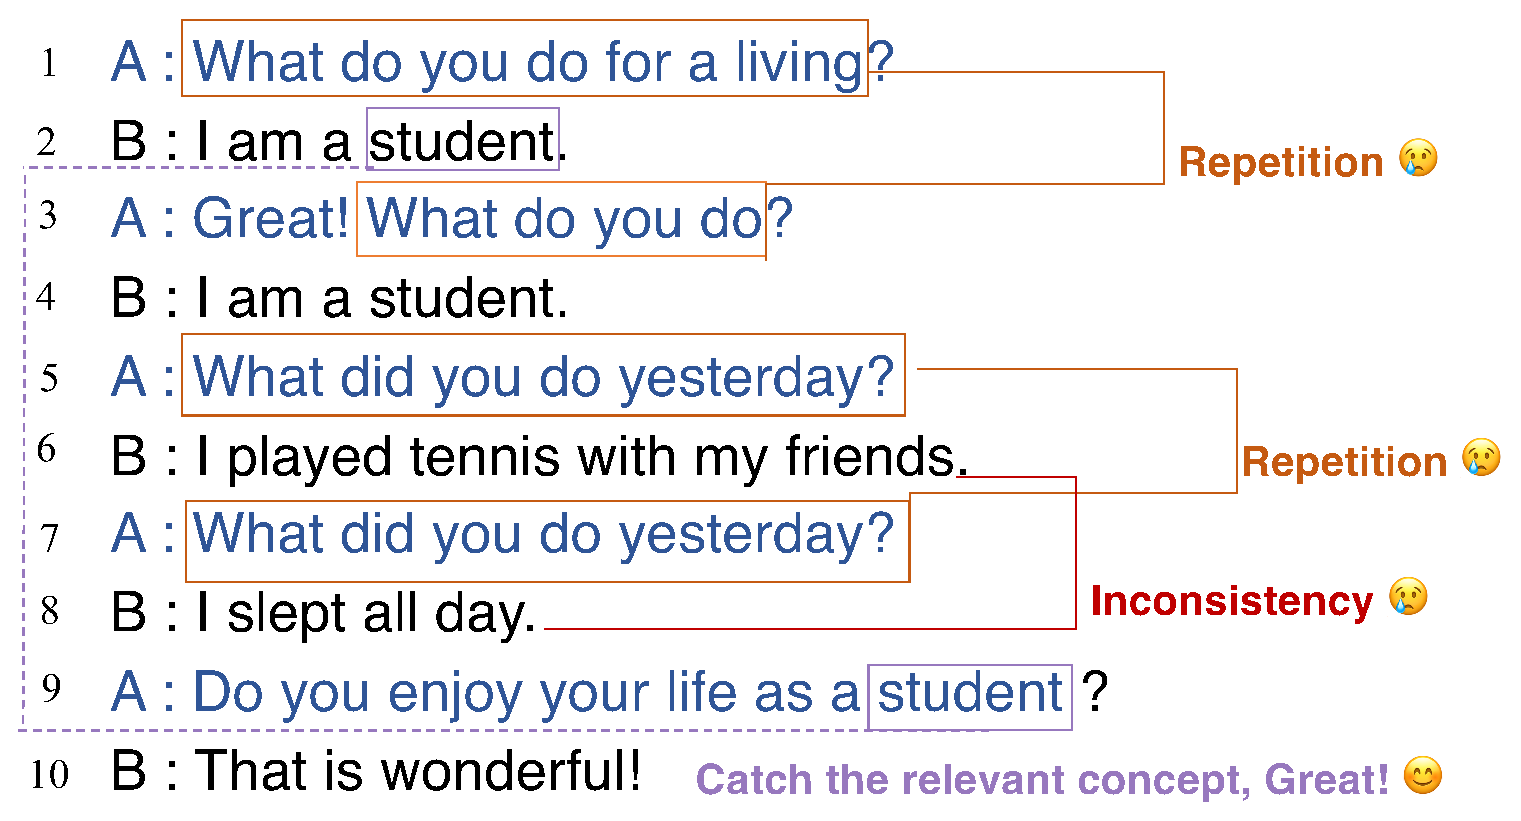
\includegraphics[width=0.95\columnwidth]{example2.eps}
        \caption{A chat snippet between two bots.}
        \label{fig:example}
\end{figure}

Fluency, Knowledge, Proactivity and Specificity are scored for each turn separately
and aggregated at the end of the conversation.
Detection for diversity, consistency and relevance are more involved and are explained
using \figref{fig:example}. 

As for diversity, at each turn $t$, we first check if there exists any repetitive question.  
We can easily find turn 3 and turn 7 repeated turn 1 and turn 5 
respectively. They will then be penalized one point for repetition. 
Repetition is not penalized if the previous turn is already 
marked as a repetitive question. For example, in \figref{fig:example}, 
although turn 4 is considered a repetition of turn 2,  
we are not going to penalize it as turn 3 is a repetitive question. 

The detection of inconsistency is always triggered after the detection of repeated questions. 
If the answers to the same questions are different, we will penalize the current turn, 
such as turn 8 in \figref{fig:example}.

We decide a repetition or an inconsistency by calculating the similarity of the two turns. 
We use a similarity function to complete the calculations, which we will 
discuss in \secref{sec:experiment}. The actual diversity and consistency scores
are the negation from the amount of repetition and inconsistency.

Relevance is assessed as a bonus to reward
a bot if it is able to memorize the important relevant concepts that have shown up 
before in the conversation. We sort the concepts that have shown up in 
chat history by their IDF scores. For example, in turn 9, $A$ 
mentions the concept word ``student'' presented by $B$ in turn 2. With this
turn, $A$ will win a bonus point.


The algorithms and notations for computing diviersty, consistency and relevance are included
in \tabref{tab:functions}, \algoref{algo:rep}, \algoref{algo:inconsist}, and \algoref{algo:bonus}. 

\begin{table}[th]
\centering
\small
\begin{tabular}{c|l}
%\hline
\toprule
\textbf{Notation} & \textbf{Description} \\ \midrule
$t$ & Current turn \\
$H(t)$  &  a list of history turns prior to $t$ \\
$Sim(x,y)$ & similarity between two turns $x$ and $y$ \\
$\sigma_r$ & Threshold for detecting repetition \\
$\sigma_c$ & Threshold for detecting consistency \\
$r$ & Weight for repetition \\
$c$ & Weight for inconsistency \\
$b$ & Weight for bonus \\
$d$ & Min distance between consecutive mentions \\
IDF list & List of lemma in chatlog sorted by IDF\\
$p$ & Percentage of important lemmas in IDF list\\
$R(t)$ &  Repetition penalty for turn $t$ \\
$C(t)$ &  Inconsistency penalty for turn $t$ \\ 
$B(t)$ &  Memory bonus for turn $t$ \\
$Rep(t)$ & A list of repeated turns for turn $t$ \\  
\bottomrule
\end{tabular}
\caption{
Functions and variables in algorithms.}
\label{tab:functions}
\end{table}

\begin{algorithm}[th]
\small
\caption{Scoring for Diversity}
\label{algo:rep}
\hspace*{0.02in} {\bf Input:}
 $t$, $H$, $Sim$, $\sigma_{r}$
; \hspace*{0.02in} {\bf Output: } 
 $R$;
\begin{algorithmic}[1]
\State //Starting to detect repetition
\For {$u$ in $H(t)$}
	\If {$Sim(t,u) \geq \sigma_{r}$}
		\State Add $u$ to $Rep(t)$
	\EndIf
\EndFor
    \If{$len(Rep(t))\geq 0$}
        \If{$t$ is a question and We can find a question in $Rep(t)$}
        \State $ R(t) \leftarrow  R(t) + 1$ 
        \Else
        \If {the previous turn of $t$ is not a repetitive question}
        \State $R(t)) \leftarrow R(t) + 1$ 
        \EndIf
        \EndIf
    \EndIf
\end{algorithmic}
\end{algorithm}


\begin{algorithm}[th]
\small
\caption{Scoring for Consistency}
\label{algo:inconsist}
\hspace*{0.02in} {\bf Input:}
$t$, $H$, $Sim$, $\sigma_{c}$
; \hspace*{0.02in} {\bf Output:  } 
 $C$;
\begin{algorithmic}[1]
\State // Inconsistency detection
 \If {previous turn of $p$ is a repetitive question} 
   \If{ the response $res$ to the question repeated by turn $p$ contradicts turn $i$ with $Sim(t, res) \leq \sigma_{c}$ }
    \State $C(t) \leftarrow C(t) + 1$
   \EndIf
  \EndIf
\end{algorithmic}
\end{algorithm}

\begin{algorithm}[th]
\small
\caption{Scoring for Relevance}
\label{algo:bonus}
\hspace*{0.02in} {\bf Input:}
$t$, $p$, $d$
; \hspace*{0.02in} {\bf Output:  } 
$B$;
\begin{algorithmic}[1]
\State // Assessing the ability of catching relevant concepts\\
$B(t) \leftarrow 0$
\For {all tokens $tk$ in current turn $t$}
 \If {$t$ - previous occurrence turn of $tk > d$ and $tk$ in the top $p\%$ of the IDF list of all tokens in the dialogue} 
   \State $B(t) \leftarrow 1$
  \EndIf
 \EndFor
\end{algorithmic}
\end{algorithm}

At the end of each game, each bot gets seven scores, one for each dimension.  
After pairwise comparison on individual dimension, a bot gains one point for win and zero point for a tie or lose.
The final score of each bot is determined by the sum of their individual scores.
%\KZ{Are these scores positive or negative? Comparable between bots?}

\subsubsection*{Match-level Scoring}
%\KZ{Use an equation to compute the final scores?}
One match which consists of two games, each started with a different bot, 
decides winning or losing between two bots.
For match-level scoring, we mimic the scoring rules of soccer tournament. 
For each match, $W$ points for the winner,  
$T$ points for a tie and 
$L$ points for the loser.
The value of $W$, $T$ and $L$ will be discussed in \secref{sec:ablation}. 

%\KZ{At the match level, we need to consider different starting context for the bots? I think we should present a few options for the reader and say that we are limited to these.}

\subsubsection*{Tournament-level Scoring}
%\KZ{Use an equation to compute the final scores?}
We count the points by simply summing up their scores gained in every match. Currently, several bots with the same final rank are tolerated. For future study, it's possible to mimic more detailed rules presented in sports match such as determine their ranking based on their win-loss relationship in the match between them.  
If they are still tied, we could propose an “overtime” for these two bots, one human judge may observe their performance and then make the decision of the game.

\section{Experiment}
In this section, we experiment on different NLG tasks. We first present the experimental setup on different tasks. Then, we show the quantitative and qualitative results together with comprehensive analysis and ablation studies.

\subsection{Implementation Details}
We evaluate the newly proposed ICL strategy on five commonly-researched natural language generation tasks: reading comprehension, dialogue summarization, style transfer, question generation and news summarization. Details on the task description, the strong baseline, corresponding  dataset, evaluation metrics and key hyper-parameters for each task are presented as follows.

\begin{table*}[th]
	\scriptsize
	\centering
	\begin{tabular}{lp{1.1cm}rrrcccc}
		\hline
		Task & Dataset & \#Train & \#Val & \#Test & Input & Output & Avg & Std\\
		\hline
		Reading Comprehension & DREAM & 6,116 & 2,040 & 2,041 & ``Q:''+ question + dialogue & answer & 5.59 & 2.61\\
		Dialogue Summarization & SAMSum & 14,732 & 818 & 819 & dialogue & summary  & 24.99 & 13.06\\
		Style Transfer & Shakespeare & 36,790 & 2,436 & 2,924 & original/modern  & modern/original  & 11.63 & 8.19 \\
		Question Generation & SQuAD1.1 & 75,722 & 10,570 & 11,877 & passage + [SEP] + answer & question & 13.09 & 4.27 \\
		News Summarization & CNNDM & 287,227& 13,368& 11,490 & document & summary & 70.97 & 29.59\\ 
		\hline
	\end{tabular}
	\caption{A summary of tasks and datasets. \#Train, \#Val and \#Test refers to the number of samples in the corresponding dataset. Avg and Std are the statistics for the number of output tokens. ``+'' refers to the concatenation operation.}
	\label{tab:taskdata}
\end{table*}

\textbf{Reading comprehension} is the task that answering questions about a piece of text. We use the DREAM dataset~\cite{sun2019dream} where questions are about corresponding dialogues and the answer is a complete sentence in natural language. We neglect the negative choices in the original dataset and formulate it as a NLG task. We adopt the pre-trained language model BART~\cite{lewis2020bart} as the baseline, where the input is a concatenation of a question and the corresponding dialogue made up of speakers and utterances. 
We experiment with  transformers\footnote{\url{https://github.com/huggingface/transformers}} based on the publically available ``facebook/bart-large'' checkpoint \footnote{\url{https://huggingface.co/facebook/bart-large}}.
%The preceding BART model is also adopted as the baseline, whereas the input is a concatenation of question and a dialogue.
The generated answers are evaluated by BLEU scores\footnote{The BLEU-1/2/3/4 scores are computed according the Google's implementation(\url{https://github.com/tensorflow/nmt/blob/master/nmt/scripts/bleu.py}).}~\cite{papineni2002bleu} widely used for QA systems, together with Meteor and Rouge-L F1 as mentioned above. The parameters are also the same as dialogue summarization, except that the early-stop is activated if there is no improvement on the perplexity of the validation set. 


\textbf{Dialogue summarization} is to generate a concise summary covering the salient information in the input dialogue. The preceding model BART has shown to be a strong baseline for this task, where only the dialogue is concatenated into a single sequence as the input. We experiment with  %transformers\footnote{\url{https://github.com/huggingface/transformers}} based on the publically available ``facebook/bart-large'' checkpoint \footnote{\url{https://huggingface.co/facebook/bart-large}} and 
SAMSum dataset\footnote{\url{https://arxiv.org/src/1911.12237v2/anc/corpus.7z}}~\cite{gliwa2019samsum} for daily-chat dialogues. 
The generated summaries are evaluated by comparing with the reference through evaluation metrics, including Rouge-1/2/L F1 scores\footnote{\url{https://github.com/pltrdy/files2rouge}}~\cite{lin2004rouge}, Meteor~\cite{banerjee2005meteor} and BertScore F1\footnote{Both Meteor and BertScore are calculated by SummEval(\url{https://github.com/Yale-LILY/SummEval}), and the latter one is based on the default bert-base-uncased model.}. We evaluate the model on the validation set after each training epoch and the early-stop patience will be added 1 if there is no improvement according to the Rouge-2 F1 score. The training process terminates when the early-stop patience equals or is larger than 3.  During the inference, the minimum and maximum output length is set to 5 and 100 respectively, with no\_repeat\_ngram\_size=3, length\_penalty=1.0 and num\_beams=4.


% The answer is either a span of words in the original text or a complete sentence in natural language.
\textbf{Style transfer} preserves the semantic meaning of a given sentence while modifies it's style, such as positive to negative, formal to informal, etc.
We adopt the Shakespeare author imitation dataset~\cite{xu2012paraphrasing}, containing William Shakespeare's original plays and corresponding modernized versions. Krishna el al.~\shortcite{krishna2020reformulating} proposed to do unsupervised style transfer by training paraphrase models based on the GPT-2 language model~\cite{radford2019language}. We re-implemented their approach STRAT\footnote{\url{https://github.com/martiansideofthemoon/style-transfer-paraphrase}} and evaluated with the provided script. Evaluation metrics includes 
transfer accuracy(ACC), semantic similarity(SIM), Fluency(FL) and two aggregation metrics, i.e., geometric averaging(GM) and their newly introduced $J(\cdot)$ metric. The hyper-parameter $hp$ equaling 0.0, 0.6 or 0.9  in Table~\ref{tab:end2endst} is the sampling parameter for trades off between ACC and SIM in their approach. 
In the training stage, we evaluate the model after updating every 500 steps. The perplexity on the validation set is used to activate the early-stop which equals 3. The inference is done as default.
 
\textbf{Question generation}~\cite{zhou2017neural} aims at generating a question given an input document and its corresponding answer span. SQuAD 1.1~\cite{rajpurkar2016squad} is generally used for evaluation. We adopt the data split as in \cite{du2017learning} and fine-tune the pre-trained UniLM~\cite{dong2019unified} as the strong baseline according to their official implementation\footnote{\url{https://github.com/microsoft/unilm/tree/master/unilm-v1}}. Generated questions are evaluated by metrics including BLEU-1/2/3/4, Meteor and Rouge-L with the provided scripts. The model is evaluated every 1000 steps and the early-stop equaling 3 is associated with the perplexity on the validation set. Other parameters are unchanged following the official guideline.

\textbf{News summarization} differs from dialogue summarization where the input is a document instead of a dialogue. We adopt the same strong baseline BART and evaluation metrics as dialogue summarization. Experiments are done with CNNDM dataset~\cite{HermannKGEKSB15} consisting of news articles and multi-sentence summaries\footnote{\url{https://github.com/pytorch/fairseq/blob/main/examples/bart/README.summarization.md}}. The model is evaluated every 2000 steps and the early-stop equaling 3 is associated with the Rouge-2 on the validation set. During the inference, the minimum and maximum output length is set to 45 and 140 respectively, with no\_repeat\_ngram\_size=3, length\_penalty=2.0 and num\_beams=4.
%\footnote{Inference parameters are borrowed from \url{https://github.com/pytorch/fairseq/blob/main/examples/bart/summarize.py}}

The summary of each task is listed in Table~\ref{tab:taskdata}. For fair comparisons, we re-implemented baselines following the above instructions on our machine. On top of the above baselines, we further arm them with the ICL strategy according to the Algorithm~\ref{alg:picl}. The settings of newly introduce Start and Stride are specified and discussed in following sub-sections. All of our experiments are done on a single RTX 3090 or a single RTX 2080Ti with 24G and 11G GPU memory respectively.
%and the result are averaged over three runs.


 
\subsection{Automatic Evaluations on Different Tasks}
\label{sec:taskperformances}

We compare our approach with the vanilla models mentioned above and the approach from~\citet{liang-etal-2021-token-wise} as baselines.
The performances on different NLG tasks are shown in Table~\ref{tab:end2end}. 
These tasks not only focus on solving different problems, but also has various amount of training data as well
as reference output lengths as shown
Table~\ref{tab:taskdata}.
Besides, the basic model are also different, including BART, GPT-2 and UniLM. 
Our new training strategy achieves significantly improvements among different tasks on most evaluation metrics, which shows that our method not only works well, but also has strong generalization abilities.

We explain the some specific results as follows:

(1) Our training strategy boosts the performances of the original STRAT with different $hp$ in the style transfer task. GM and J are two comprehensive evaluation metrics, with our approach topping the ranks with significant improvements.

(2) TCL generally performs poorly on tasks
with more training data. For example, it failed on question generation without any improvements over the vanilla model under the same parameter setting, while ICL still 
logs gains. This is mainly due to two reasons.
First, because the nature of TCL is data augmentation which is more effective in low-resource settings,
when training data is abundant, it becomes less useful. 
Second, the way they calculate the loss as sub-sequence generation better suites paraphrasing tasks, such as machine translation tested in their paper, as the order of 
the corresponding tokens between input and output 
are almost the same. Learning such forward mapping can 
be regarded as a kind of ``easy-to-hard'' 
in these limited scenarios.
However, this doesn't hold true for other tasks, 
such as summarization and question generation. 
Therefore, we didn't further test it on CNNDM since
CNNDM has the large amount of training data among
the five.

(3) For news summarization, Rouge-1 scores (precision, recall) for the baseline and our method on CNNDM are (38.16, 52.72) and (40.84, 49.23) correspondingly. Our method made substantial improvements on the precision with a compromise on the recall. 
The meteor score based on the unigram precision and recall emphasizes more on the recall than the Rouge-1 F1. As a result, it drops while Rouge-1 F1 increases. Overall, our method still outperforms BART on this task, especially on F1 scores of Rouge-2 and Rouge-L.




\begin{table}[th]
	\small
	\centering
	\begin{subtable}{\linewidth}
		\scriptsize
		\centering
		\begin{tabular}{lcccccc}
			\hline
			{Method} & {B1} & {B2} & {B3} & {B4} & {Met} & {RL}\\
			\hline
			w/o CL &  32.03 & 16.01 & 8.77 & \textbf{4.80} & 19.84 & 38.89\\
			TCL & 32.53 & 16.25 & 8.52 &4.67 &19.88 & 39.65 \\
			ICL &  \underline{\textbf{33.99}} & \underline{\textbf{17.43}} & \underline{\textbf{9.18 }}& 4.64 & \textbf{20.60} & \textbf{40.78}\\

			\hline
		\end{tabular}
		\caption{Reading Comprehension}
		\label{tab:end2endrc}
	\end{subtable}
	\\[5pt]
	\begin{subtable}{\linewidth}
		\scriptsize
		\centering
		\begin{tabular}{lccccc}
			\hline
			{Method} & {R1} & {R2} & {RL} & {Met} & {BertS} \\
			\hline
			%BART & 52.60&27.00 &42.10 &- & - \\
			w/o CL & 51.88 & 27.30 & 42.77 & 24.75 & 71.38 \\
			TCL  & 52.33 & 27.80 & \textbf{43.91} & 24.59 & 71.77 \\
			ICL & \underline{\textbf{53.07}} & \underline{\textbf{28.23}} & {43.83} & \underline{\textbf{26.12}}& \underline{\textbf{72.17}} \\
			
			\hline
		\end{tabular}
		\caption{Dialogue Summarization}
		\label{tab:end2endds}
	\end{subtable}
	\\[5pt]
	\begin{subtable}{\linewidth}
		\scriptsize
		\centering
		\begin{tabular}{lcccccc}
			
			\hline
			{Method}&$hp$ &  {ACC} & {SIM} & {FL} & {GM} & {J}\\
			\hline
			%\multirow{3}{*}{STRAT}& 0.0 & 71.70 & \textbf{56.40} & 85.20 & 70.10 & 34.70 \\
			%& 0.6 & 75.70 & 53.70 & 82.70 & 69.50 & 33.50 \\
			%& 0.9 & 79.80 & 47.60 & 71.70 & 64.80 & 27.50 \\
			%\hline
			\multirow{3}{*}{w/o CL}& 0.0 & 70.49 & 55.70 & 85.98 & 69.63& 33.72 \\
			& 0.6 &75.31 & 53.46 & 82.56 & 69.27& 33.30\\
			& 0.9 & 78.76 & 47.38 & 74.42 &65.24 & 27.88\\
						\hline
			\multirow{3}{*}{TCL } & 0.0 & 70.31 & \textbf{55.95} &\textbf{87.24} &  70.01& 34.71 \\
			& 0.6 & 74.79 & 53.14 & 82.56 & 68.97 & 33.21 \\
			& 0.9 & 79.41 & 46.88 & 71.92 &64.45 & 26.92 \\
			\hline
			\multirow{3}{*}{ICL}& 0.0 & \underline{73.72} & 55.91 & 86.30 & \underline{\textbf{70.60}} &\underline{\textbf{35.81}}\\
			& 0.6 & 77.26 & \underline{53.80} & \underline{83.87} & \underline{70.38} & 34.64\\
			& 0.9 & \textbf{79.65} & 48.16 & 76.06 & 66.32 & 29.03\\

			\hline
		\end{tabular}
		\caption{Style Transfer.}
		\label{tab:end2endst}
	\end{subtable}
	\\[5pt]
	\begin{subtable}{\linewidth}
		\scriptsize
		\centering
		\begin{tabular}{lcccccc}
			\hline
			{Method} & {B1} & {B2} & {B3} & {B4} & {Met} & {RL}\\
			\hline
			w/o CL & \textbf{50.38} & 35.67 & 27.24 & 21.36 & 24.40 & 50.67 \\
			TCL &\textbf{50.38} & 35.67 & 27.24 & 21.36 & 24.40 & 50.67\\
			ICL &  50.18 & \textbf{35.72} & \textbf{27.36} & \textbf{21.54} & \textbf{24.57} & \underline{\textbf{51.09}} \\
			\hline
		\end{tabular}
		\caption{Question Generation}
		\label{tab:end2endqg}
	\end{subtable}
		\\[5pt]
	\begin{subtable}{\linewidth}
		\scriptsize
		\centering
		\begin{tabular}{lccccc}
			\hline
			{Method} & {R1} & {R2} & {RL} & {Met} & {BertS}\\
			\hline
			%BART &  \\
			w/o CL &  43.07 & 20.01 & 35.94 & \textbf{21.44} & 63.72 \\
			TCL & - & -&- &- &- \\
			ICL & \textbf{43.39} & \underline{\textbf{20.55}} & \underline{\textbf{36.63}} & 19.68 & \textbf{64.05}\\
			\hline
		\end{tabular}
		\caption{News Summarization}
		\label{tab:end2endns}
	\end{subtable}
	\caption{Performances on different NLG tasks. ICL represents the models trained with our ICL algorithm. TCL refers to the previous work from~\cite{liang-etal-2021-token-wise}. Scores underlined are statistically significantly better than both re-implemented baselines with $p<0.05$ according to t-test. }	
	\label{tab:end2end}
\end{table}


\subsection{Human Evaluations}

To further prove the improvement of ICL, we hired three proficient English speakers for human evaluation. 20 samples from the test set of each task are randomly selected, ignoring the ones with totally same generations among three models, including the vanilla model, TCL and ICL. The original input, reference output and three generations are shown to annotators together, while the order of three generations are unknown and different among samples. 3-point Likert Scale is adopted for scoring for each generation~\cite{gliwa2019samsum}, where [1, 3, 5] represent 
excellent, moderate and disappointing results 
respectively. The average scores and agreements 
among the annotators are shown in 
Table~\ref{tab:humaneval}.

The Fleiss Kappa on the first four tasks indicates the fair to moderate agreements. It shows the promising improvement of ICL over the vanilla model and TCL especially on DREAM, SAMSum, and SQuAD1.1, which is consistent with the conclusion based on automatic metrics.
Although the agreement on style transfer is fair, 
our annotators without Shakespeare background 
tend to give low scores to all outputs.
Therefore, the absolute improvement is 
only $0.04$ compared to both baselines.
%This mainly due to the indistinguishable styles between
%Shakespeare’s plays with are quite different from modern languages. 
Besides, the poor agreement on CNNDM reflects the 
diverse concerns of summarization from different 
annotators. Without more specific instructions, they 
tends to focus more on the content coverage instead 
of checking the detailed facts. This is also 
consistent with the higher Meteor scores of the 
vanilla model over ICL.

\begin{table}[th]
	\scriptsize
	\centering
	\begin{tabular}{l|ccc|c}
		\hline
		{Datasets} & {w/o CL} & {TCL} & {ICL} & {Agreement}  \\
		\hline
		DREAM  &3.07 & 2.50&3.20 &0.48 \\
		SAMSum &2.97 &3.57 &3.97 &0.40 \\
		Shakespeare &2.23 &2.23 & 2.27&0.32 \\
		SQuAD1.1 &3.43 & 3.43 &3.77 &0.35 \\
		CNNDM & 3.45 &- &3.40 &0.11 \\
	%	\hline
	%	overall & & & &\\
		\hline
	\end{tabular}
	\caption{Human evaluations. The agreement is calculated by Fleiss Kappa.}
	\label{tab:humaneval}
\end{table}




%Following Liu et al.\shortcite{liu2021competence}'s work, we asked annotators to comparing the performance between our generated results and baselines by choosing from ``Better, Tie, Worse''. 
%The counts for each choice are shown in Table~\cite{}, where the Fleiss Kappa among annotators is ??.

%Analysis





%\subsection{Analysis on Variable Generation Lengths}

%Teacher forcing, which predicts each token given the reference summary tokens during training and given the previous generated tokens during inference, leads to the exposure bias problem for NLG tasks.
%Since ICL starts the training process by predicting the last few tokens of outputs and gradually calculates the loss based on more tokens when the model is stronger, we hypothesis that it can alleviate the exposure bias for training Seq2Seq models to some extent.
%As stated in~\cite{pang2020text}, the output quality tends to degrade as the output length increase with the exposure bias.
%So, we divided the test set of each task according to the length of the generated output into 4 buckets and randomly picked 20 samples in each buckets for both the corresponding baselines and our approach. Each generation is annotated by 5 point Likert Scale, where 1 is the worst and 5 is the best. 

%The trends of performances on variable generation lengths are in Figure~\ref{}.


% \vspace{-1em}
\section{Related Work} \label{rw}

%\subsection{Legal Judgment Prediction}

Legal Judgment Prediction (LJP) aims to predict the outcomes of legal cases~\cite{chalkidis-etal-2019-neural, an-etal-2022-charge}. These predictions encompass the charges, applicable statutory provisions, and suggested sentencing, including prison terms. Previous studies have predominantly framed these tasks as classification problems. There are three main approaches in LJP research~\cite{DBLP:journals/access/CuiSW23}.

\textbf{Content-based models.} 
These models employ language models to extract semantic features from the case documents and make predictions via MLP or linear layer. BERT~\cite{devlin-etal-2019-bert} and Electra~\cite{DBLP:conf/iclr/ClarkLLM20} stand out as representative language models in the literature. These models can be trained on large corpora. However, recent studies showed that language models may not be as effective in legal judgment prediction tasks compared to large language models, specifically GPT-3 and GPT-4~\cite{shui-etal-2023-comprehensive, wu-etal-2023-precedent}. These findings suggest that the legal domain problems are quite complicated so merely applying a language model does not guarantee high performance~\cite{vats-etal-2023-llms}.

\textbf{Models learning from historical cases.} 
Inspired by case law principles, these models aim to extract valuable insights from historical cases to enhance the prediction accuracy for new cases~\cite{DBLP:conf/cicai/ZhouLWKZW22}. Case relations can be learned by node classification of a graph~\cite{Rformer}, or contrastive learning~\cite{liu-etal-2022-augmenting}. 

\textbf{Models enhanced by legal knowledge.} 
Unlike other models, these models leverage extra legal knowledge. The legal knowledge utilized can be the content of legal rules~\cite{ML-LJP} or the judicial process~\cite{DBLP:conf/emnlp/ZhongGTX0S18,deng-etal-2023-syllogistic}. An innovative example of a law-enhanced approach is RLJP~\cite{Wu2022TowardsIA}, which draws inspiration from the judicial decision-making process and introduce an intermediate step to generate rationale and use this information to the LJP. However, these works often require additional training information, such as reference rationale from judges. Incorporating statutory text directly into prediction models represents another pivotal strategy for embedding legal knowledge, enabling the models to learn directly from the law text, as demonstrated in studies~\cite{neurjudge,ML-LJP}. 

% \paragraph{Few-shot Learning} 
% Although a few prior studies acknowledge the significance of charges with limited case numbers, and claim that it is not correct to directly ignore charges with fewer than 100 cases in evaluation. However, instead of conducting a detailed few-shot analysis~\cite{DBLP:conf/nldb/ZhaoSSA17, hu-etal-2018-shot}, these studies simply lower the threshold from 100 to 10 cases. The mixed results obtained do not definitively demonstrate effectiveness in few-shot learning scenarios.

% \subsection{Graph Representation for Text}

% Text embedding methods like Word-to-vector and Transformer-based model encoding are widely employed across a wide range of tasks in natural language processing (NLP), including Legal Judgment Prediction (LJP)~\cite{Greco2023BringingOI}. These techniques have been foundational in advancing NLP applications by enabling sophisticated understanding and processing of text data. However, recent studies have identified graph representations as a particularly effective approach for capturing the structural information inherent in text. This advantage is mentioned in several tasks, such as text summarization~\cite{DBLP:conf/acl/GaoCLC00Y23} and legal case classification~\cite{wang-etal-2022-d2gclf}, etc.


\section{Conclusion}

In this study, we conducted a comprehensive analysis of Prison Term Prediction (PTP) and identified two major issues: structural representation of legal knowledge and the scarcity of training data for most crimes. To address these issues, we proposed a novel approach, \lawgraph{}, to represent the structural legal knowledge. We further proposed a lightweight Statute Knowledge Encoder (SKE) for end-to-end training of our model. We performed extensive experiments to compare SKE with previous works and LLMs. The experimental results have indicated the superiority of SKE over previous works. 

\section*{Limitations}
We introduced a new method to transform plain text statute information into law graphs, aiming to enhance the performance of predictors in predicting prison terms. Our research demonstrated that our proposed construction process can produce law graphs with an average accuracy of 97\%. However, we observed that errors in the law graph can impact the performance of the predictor, while the rate of error is small.
Furthermore, the potential of our law graph to improve performance in other legal tasks and in cases involving multiple crimes has not been thoroughly investigated. These two aspects will be the primary focus of our future research.




\section*{Ethic Statement}
\paragraph{Privacy Concerns.} The cases analyzed in this paper are sourced from the open dataset CAIL2018, which has been widely utilized in prior research. Given that these cases are published on China Judgment Online and have been anonymized, the risk of disclosing personal information about the individuals involved is minimal. Nonetheless, to enhance privacy protection and adhere to ethical standards, we will only release the case indices, not the full text of the cases.

\paragraph{Individual Affected Concerns.} While our proposed methods can achieve some improvements compared to previous research, there is still a gap in achieving flawless prediction. We highly respect and understand that if the proposed methods are used in the real world, incorrect predictions may cause serious consequences. We want to highlight that this is only a forward step in this research topic; we have no intent to implement the predicted model in actual court settings immediately. 

\paragraph{Responsible Usage.} At this stage, the proposed methods still have some limitations. We do not recommend that any users blindly trust the model's output. The output may be seen as a suggestion, but the final legal opinion should be made by professional legal experts. Users should be aware that errors may exist in the output. Besides, any use of this tool as legal advice should comply with local laws and administrative regulations.

% Bibliography entries for the entire Anthology, followed by custom entries
%\bibliography{anthology,custom}
% Custom bibliography entries only
\bibliography{custom}

\appendix
% \section{Example of Nodes and Edge in \lawgraph{}}
\label{ne}

Table~\ref{tab:node-example} and \ref{tab:edge-example} shows the example of node and edge used in the proposed \lawgraph{}.

\begin{table}
    \centering
    \tiny
    \caption{Node types in \lawgraph{}}
    \begin{tabular}{c|p{0.3\columnwidth}|p{0.4\columnwidth}}
    \hline
    \hline
        Entity Type & Definition & Example(s)  \\
        \hline
        \textit{Law\_keyword} & A law keyword is the description selected from the law article, it can be either a word or a phrase. & \textit{Defendant; Extremely Huge Amount; Other Especially Serious Circumstances; Using Fake Economic Contracts}\\
        \hline
        \textit{Law\_punishment} & A law punishment represents sanction in legal norm. & \textit{Fixed-Term Imprisonment; Fine; Detention}\\
        \hline
        \textit{Law\_numerical} & An law numerical represents a limit on the amount of a description or punishment. & \textit{>= Twenty Thousand Yuan; <= Ten Years; <= Five Hundred Thousand Yuan}\\
        \hline
        \textit{Logic} & \textit{Not} represents The left node has an inverse relation to the right node. 
        
        \textit{And} represents the father node depends on all children nodes. 
        
        \textit{Or} represents the father node depends on one of the children nodes. & \textit{AND ${\stackrel{Satisfy}\longrightarrow}$ AND ${\longleftarrow}$ (1) Fixed Term Imprisonment; (2) Fine.}
        \textit{Fraud Loans from Banks ${\longleftarrow}$ OR ${\stackrel{Constrain}\longleftarrow}$ (1) Using Fake Certification Documents; (2) Using Fake Economic Contracts.}\\
        \hline
        \hline
    \end{tabular}
    \label{tab:node-example}
\end{table}

\begin{table}
    \centering
    \tiny
    \caption{Edge types in \lawgraph{}.}
    \label{tab:edge-example}
    \begin{tabular}{p{0.1\columnwidth}|p{0.3\columnwidth}|p{0.15\columnwidth}|p{0.2\columnwidth}}
    \hline
    \hline
        Relation & Definition & Example Sentences &Logic expression\\ 
        \hline
        \textit{Do} & Describe: A type of normal Behaviors; Domain: Instance; Range: All type of Entities & A borrowed money. & \textit{A ${\stackrel{Do}{\longrightarrow}}$ borrow}\\
        \hline
        \textit{Effect} & Describe: A type of influence; Domain: Instance; Range: All type of Entities & A stolen B's money.& \textit{stolen ${\stackrel{Effect}{\longrightarrow}}$ B's money}\\
        \hline
        \textit{Define} & Describe: Defined by Law terminology; Domain: All type of Entities; Range: Law\_concept & Computer system means a computer. & \textit{Computer ${\stackrel{Define}{\longrightarrow}}$ Computer \ system}\\
        \hline
        \textit{Satisfy} & Describe: Meet the Law article; Domain: Law\_concept; Range: All type of Entities & The ground is satisfied that B.  & $ Ground \stackrel{Satisfy}{\longrightarrow} B;$\\
        \hline
        \textit{Consider} &
        Describe: Considered by Judge; Domain: Law\_concept; Range: All type of Entities & The ground should consider B. & $ Ground \stackrel{Consider}{\longrightarrow} B;$\\
        \hline
        \textit{Part\_of} &
        Describe: Be a subset in Law; Domain: All type of Entities Range: All type of Entities & 
        Mr W dissolves his marriage.  & $ Mr \ W \stackrel{PartOf}{\longrightarrow} marriage$\\
        \hline
        \hline
    \end{tabular}
\end{table}
% \section{Details of \lawgraph{} Construction}
\label{dcon}

\begin{algorithm}
\small
\caption{Integration of \lawgraph{} \KZ{This pseudo code is not necessary, cut it.}}
\label{alg:Integration}
\begin{algorithmic}[1]
\Require Completed all four parsing processes
\Ensure Generate a completed \lawgraph{}
\State $\mathcal{E} \gets \mathcal{E} \bigcup \{(A, Root of DP, ConstraionRelation)\}$ \Comment{Connect the root of \lawgraph{}-DP with \( A \)}
\State $\mathcal{V} \gets \mathcal{V} \bigcup$ \Comment{Generate logic nodes  AND for each \lawgraph{}-SP, and link by \( SatisfyRelation \)}
\State Connect \( A \) to each \( AND \), and connect each branch to their corresponding \( AND \)
\end{algorithmic}
% \vspace{-1em}
\end{algorithm}


\begin{algorithm}[!t]
\small
\caption{Hypothesis Parser (HP)}
\label{alg:HP}
\begin{algorithmic}[1]
\Require The hypothesis $H$ of statutory provisions
\Ensure Parse \( H \) into nodes $\mathcal{V}_{HP}$ and relations $\mathcal{E}_{HP}$.
\State $I$, $O$ <- Segment hypothesis $H$ through \textit{word matching} \Comment{\textit{flag words} $\in \{\text{;, :, etc.}\}$}
\State $A$ <- Extract subject-verb and object from $I$ through LTP
\State $\mathcal{V}_{HP} \gets [A] $
\State $D$ <- Generate a keyword node named ``Defendant''
\State $\mathcal{V}_{HP} \gets \mathcal{V}_{HP} \bigcup D$
\State $\mathcal{E}_{HP} \gets \mathcal{E}_{HP} \bigcup (D, DoRelation, A)$
\If{\( I \) contains basic conditions \( M^b \)} \Comment{Conditions $\in$ \{\( location, motivation, time \)\}}
\State \( M^b_X \) <- Extract Purpose Adverbial, Time Adverbial from $I$ through LTP \Comment{$X$ could be one of the motivation $v$, time $t$}
\State $\mathcal{V}_{HP} \gets \mathcal{V}_{HP} \bigcup [M^b_X$]
\State $\mathcal{V}_{HP} \gets \mathcal{V}_{HP} \bigcup M^b_p$
\State $\mathcal{E}_{HP} \gets \mathcal{E}_{HP} \bigcup [M^b_X, ConstrainRelation, A]$
\State $\mathcal{E}_{HP} \gets \mathcal{E}_{HP} \bigcup (A, ModifyRelation, M^b_p)$
\EndIf
\If{\( H \) contains \( O \)}
\State $\mathcal{V}_{HP} \gets [{OR}_0]$ \Comment{Set ${OR}_0$ is the root node}
\State $O_n$ <- split \( O \) into a list \( O_1, O_2, \cdots, O_i \) through word matching \Comment{\textit{flag words} $\in \{\text{(1), ;, etc.}\}$}
\State Connect the root of \( O \) to \( A \) by \(ContrainRelation\)
\For{$i=1$ \textbf{to} $N$} \Comment{$N$ = Count($O$)}
\State $\mathcal{V}_{O_i} \gets [R_{O_i}]$ \Comment{$R_{O_i}$ is the root node of $O_i$, and is either $OR$ or $AND$ node.}
\State $E_{O_i}$, $K_{O_i}$ <- Extract effect node and keyword node from $O_i$ through LTP and word matching
\State $\mathcal{V}_{O_i} \gets \mathcal{V}_{O_i} \bigcup E_{O_i}$
\State $\mathcal{V}_{O_i} \gets \mathcal{V}_{O_i} \bigcup K_{O_i}$
\State $\mathcal{E}_{O_i} \gets \mathcal{E}_{O_i} \bigcup (E_{O_i}, Relation, K_{O_i})$ \Comment{The relation could be \(EffectRelation\), \(ContrainRelation\) or \(LeadToRelation\)}
\State $\mathcal{E}_{O_i} \gets \mathcal{E}_{O_i} \bigcup (K_{O_i}, DefaultRelation, R_{O_i})$
\State $\mathcal{V}_{HP} \gets \mathcal{V}_{HP} \bigcup \mathcal{V}_{O_i}$
\State $\mathcal{E}_{HP} \gets \mathcal{E}_{HP} \bigcup \mathcal{E}_{O_i}$
\EndFor
\EndIf
\end{algorithmic}
\end{algorithm}


\begin{algorithm}
\small
\caption{Disposition Parser (DP)}
\label{alg:DP}
\begin{algorithmic}[1]
\Require The disposition \( D \) of statutory provisions
\Ensure Parse \( D \) into nodes $\mathcal{V}_{DP}$ and relations $\mathcal{E}_{DP}$.
\State $\mathcal{V}_{DP} \gets [{OR}_0] $ \Comment{Set ${OR}_0$ is the root node}
\State $\mathcal{E}_{DP} \gets [ \ ] $
\For{$i=1$ \textbf{to} $N$} \Comment{$N$ = Count($D$)}
    \State Logic Node $\gets$ \textit{Generate nodes}(\( D_i \)) by word matching
\State $K_{Di} \gets$ Extract keyword nodes (\( D_i \)) by 
\State $\mathcal{E}_{DP} \gets \mathcal{E}_{DP} \bigcup (K_{Di}, DefaultRelation, {OR}_0)$
\State $\mathcal{V}_{DP} \gets \mathcal{V}_{DP} \bigcup K_{Di}$
\EndFor
\end{algorithmic}
\end{algorithm}


\begin{algorithm}
\small
\caption{Sanction Parser (SP)}
\label{alg:SP}
\begin{algorithmic}[1]
\Require The sanction \( S \) of statutory provisions
\Ensure Parse \( S \) into nodes $\mathcal{V}_{SP}$ and relations $\mathcal{E}_{SP}$.
\For{$i=1$ \textbf{to} $N$} \Comment{$N$ = Count($S$)}
\State $\mathcal{V}_{S_i} \gets [R_{S_i}]$ \Comment{$R_[S_i]$ is the root node of $S_i$, and is either $OR$ or $AND$ node.}
\State $P \gets $ Extract punishment nodes from \( S_i \) through word matching
\State $\mathcal{E}_{SP} \gets [P_i, DefaultRelation, R_{S_i}]$ 
\State  $U$ and $L \gets $ Extract comparison nodes($P_i$) \Comment{$U$ and $L$ denote upper and lower limits, respectively.}
\State $\mathcal{E}_{SP} \gets \mathcal{E}_{SP} \bigcup [U, DefaultRelation, AND]$
\State $\mathcal{E}_{SP} \gets \mathcal{E}_{SP} \bigcup  [L, DefaultRelation, AND]$ 
\State $\mathcal{V}_{SP} \gets \mathcal{V}_{SP} \bigcup [AND, U, L]$ 
\State $\mathcal{E}_{SP} \gets \mathcal{E}_{SP} \bigcup  [AND, ConstrainRelation, _]$ 
\EndFor
\State $\mathcal{V}_{SP} \gets [\mathcal{V}_{S_1},\mathcal{V}_{S_2},...,\mathcal{V}_{S_n}]$
\State $\mathcal{E}_{SP} \gets [\mathcal{E}_{S_1},\mathcal{E}_{S_2},...,\mathcal{E}_{S_n}]$
\end{algorithmic}
% \vspace{-1em}
\end{algorithm}
\section{Case Study of Law Graph}
\label{sec:a}
In this section, we apply the proposed law graph construction process in Section~\ref{con} to parse the Crime of Loan Fraud, Article 193 of the Criminal Law of China (shown in Table \ref{tab:three}), into a law graph.

\begin{figure}[H]
    \centering
    \includegraphics[width=1\linewidth]{figs/HP-Result.pdf}
    \caption{Result of Hypothesis Parser on the Crime of Loan Fraud}
    \label{fig:HP-Result}
\end{figure}

\textbf{Hypothesis Parser (HP).} In terms of \textit{hypothesis}, the target is to find the illegal conduct (\( I \)) and any related conditions (\( M \)) of the conduct in the statutory provision. For the example in Table \ref{tab:three}, we obtain the following vertices and edges:
% with Algorithm \ref{alg:HP}:
\begin{itemize}
    \item Conduct Node $A$: \textit{Fraud Loans from Banks or Other Financial Institutions}
    \item Defendant Node $D$: \textit{Defendant}
    \item Motivation Node $M_v$: \textit{Illegal Possession}
    \item Other Conditions $M_o$: \textit{Using Fake Certification Documents}; \textit{Using Fake Economic Contracts}; \textit{Fabricating False Reasons for Introduction of Capital}; \textit{Fabricating False Reasons for Projects}; \textit{Repeatedly pledging beyond the value of collateral}; and \textit{Using fake property rights certificates as collateral}.
\end{itemize}

\begin{figure}[H]
    \centering
    \includegraphics[width=1\linewidth]{figs/DP-Result.pdf}
    \caption{Result of Disposition Parser on the Crime of Loan Fraud}
    \label{fig:DP-Result}
\end{figure}

\textbf{Disposition Parser (DP).} 
% As is outlined in Algorithm \ref{alg:DP}, disposition 
The parser aims to extract all severity information from the statutory law. For the example in Table \ref{tab:three}, we obtain the following vertices and edges:

\begin{itemize}
    \item $D_1$: \textit{Large Amount}
    \item $D_2$: \textit{Huge Amount} OR \textit{Other Serious Circumstances}
    \item $D_3$: \textit{Extremely Huge Amount} OR \textit{Other Especially Serious Circumstances}
\end{itemize}


\begin{figure}[H]
    \centering
    \includegraphics[width=1\linewidth]{figs/SP-Result.pdf}
    \caption{Result of Sanction Parser on the Crime of Loan Fraud}
    \label{fig:SP-Result}
\end{figure}

\begin{figure*}
    \centering
    \includegraphics[width=0.98\linewidth]{figs/Loan Fraud Law Graph.png}
    \caption{Law-Graph on Crime of Loan Fraud}
    \label{Law-Graph-Case-study}
    \vspace{-1em}
\end{figure*}

\textbf{Sanction Parser (SP).}  
% Algorithm \ref{alg:SP} shows the process that .
SP parses all sanctions into \lawgraph{}. In this example, we obtain the following vertices and edges:
\begin{itemize}
    \item $P_1$: \textit{Fixed-term Imprisonment};
    \item $P_2$: \textit{Detention};
    \item $P_3$: \textit{Fine};
    \item $P_4$: \textit{Fixed-term Imprisonment};
    \item $P_5$: \textit{Fine};
    \item $P_6$: \textit{Fixed-term Imprisonment};
    \item $P_7$: \textit{Life Imprisonment};
    \item $P_8$: \textit{Fine};
    \item $P_9$: \textit{Confiscation of Property};
    \item $U_1$ and $L_1$: \textit{$\leq$ Five Years},  Not applicable;
    \item $U_2$ and $L_2$: Not applicable, Not applicable;
    \item $U_3$ and $L_3$: \textit{$\leq$ Two Hundred Thousand Yuan}, \textit{$\geq$ Twenty Thousand Yuan};
    \item $U_4$ and $L_4$: \textit{$\leq$ Ten Years}, \textit{$\geq$ Five Years};
    \item $U_5$ and $L_5$: \textit{$\leq$ Five Hundred Thousand Yuan};, \textit{$\geq$ Fifty Thousand Yuan};
    \item $U_6$ and $L_6$: Not applicable, \textit{$\geq$ Ten Years};
    \item $U_7$ and $L_7$: Not applicable, Not applicable;
    \item $U_8$ and $L_8$: \textit{$\leq$ Five Hundred Thousand Yuan}, \textit{$\geq$ Fifty Thousand Yuan};
    \item $U_7$ and $L_7$: Not applicable, Not applicable.
\end{itemize}




After obtaining these nodes, we utilize the edge definition (Table~\ref{tab:edge})
% and Algorithm \ref{alg:HP} to \ref{alg:Integration} 
to connect these nodes. Then, we can get the complete law graph of the Crime of Loan Fraud, Article 193 of the Criminal Law of China, shown in Figure~\ref{Law-Graph-Case-study}. After construction, we can identify the source nodes and output nodes in the \lawgraph{}, including
\begin{itemize}
    \item Source nodes: \textit{Large Amount}, \textit{Huge Amount}, \textit{Other Serious Circumstances}, \textit{Extremely Huge Amount}, \textit{Other Especially Serious Circumstances}, \textit{Defendant}, \textit{Illegal Possession}, \textit{Using Fake Certification Documents}, \textit{Using Fake Economic Contracts}, \textit{Fabricating False Reasons for Introduction of Capital}, \textit{Fabricating False Reasons for Projects}, \textit{Repeatedly pledging beyond the value of collateral}, and \textit{Using fake property rights certificates as collateral};
    \item Output nodes: \textit{AND$_1$}, \textit{AND$_2$}, and \textit{AND$_3$}.
\end{itemize}





\begin{table}
    \centering
    \scriptsize
    \caption{Prompt Template of ChatGPT for predicting prison terms. $N$ denotes the number of training samples.}
    \begin{tabular}{p{0.1\textwidth}|p{0.35\textwidth}}
    \toprule
       \multirow{2}{*}{Example 1}  & Case Fact: <demo facts>\\
       & In the absence of mentioned circumstances, presumed nonexistence, based on the aforementioned facts, the judgment is:<demo label>\\
       \multirow{1}{*}{Example $\cdots$}  & Case Fact: <demo facts>\\
       & In the absence of mentioned circumstances, presumed nonexistence, based on the aforementioned facts, the judgment is:<demo label>\\
       \multirow{2}{*}{Example N}  & Case Fact: <demo facts>\\
       & In the absence of mentioned circumstances, presumed nonexistence, based on the aforementioned facts, the judgment is:<demo label>\\
       \multirow{3}{*}{Test Case}  & Case Fact: <test facts>\\
       & In the absence of mentioned circumstances, presumed nonexistence, based on the aforementioned facts, the judgment is:\rule{1cm}{0.4pt}\\
       & Please estimate a specific length of sentence, providing only a numerical conclusion.\\
       \bottomrule
    \end{tabular}
    \label{tab:gpt_input}
\end{table}

\section{Setting Details of ChatGPT for Prison Term Prediction}
\label{sec:b}

Prompt plays a crucial role when applying LLMs to a specific task. For Prison Term Prediction (PTP) task, ChatGPT may return unexpected response, such as refusing to answer and providing rough prediction. We need to avoid these responses before evaluating the performance of ChatGPT. Inspired by the idea of in-context learning, we find it helpful to incorporate some training samples into the prompt. We then iterate through several types of prompt templates and analyze the unexpected responses. Finally, we figure out a prompt template to eliminate unexpected answers from ChatGPT, which is shown in Table~\ref{tab:gpt_input}. We use the same prompt template for ChatGPT-3.5 and ChatGPT-4.

Intuitively, the straightforward prompts can be \emph{Predict imprisonment} or \emph{Give the sentence}. Given these prompts, ChatGPT would refuse to predict the imprisonment term for reasons like \textit{Providing an exact sentencing prediction without knowing the full details of a case and the specific application of legal provisions is inaccurate. In actual judicial practice, courts consider factors such as the nature of the crime, the circumstances, the degree of harm caused to the victim, and the attitude after committing the crime to determine the sentence}.

We then modify the prompt to ask ChatGPT to ignore the content not mentioned and direcly predict the imprisonment, such as \emph{If the circumstances not mentioned are considered to be non-existent, the sentence is given}. Given this prompt, ChatGPT may return a possible imprisonment range instead of a particular number. For instance, the responses could be: \textit{In the absence of any other aggravating or mitigating circumstances, the predicted sentencing might lean towards the lighter end within the range allowed by law. Therefore, a rough estimate could be imprisonment from three to seven years, with the specific sentence being determined by the judge's discretion and the specifics of the case. Please note that this is merely a speculation based on the information provided, and the actual sentence may vary.}

We analyze the ambiguous response and manage to reach the final prompt: \emph{In the absence of mentioned circumstances, presumed nonexistence, based on the aforementioned facts, the judgment is:\rule{1cm}{0.4pt}
Please estimate a specific length of sentence, providing only a numerical conclusion.}

\end{document}
